\section{General Problem}
The problem of improving the quality of human settlements is complex and requires of a holistic approach to make effective contributions. There is a significant amount of interactions between the goals and in order to plan for a more sustainable places, these relationships need to be explored. By systematically looking at how these goals relate to each other, synergies can be enhanced, and tensions taken into consideration. Planning as a general practice will deal with evaluating and organizing what is the best course of action to meet a target. \par
%
Monitoring KPIs is an important activity, they provide information about the result of a process (or processes). By them self, they do not contain information about how a system works or is performing, but information about the working of a system are important for Planning purposes. \par
%
\begin{figure}[hbt!]
    \centering
    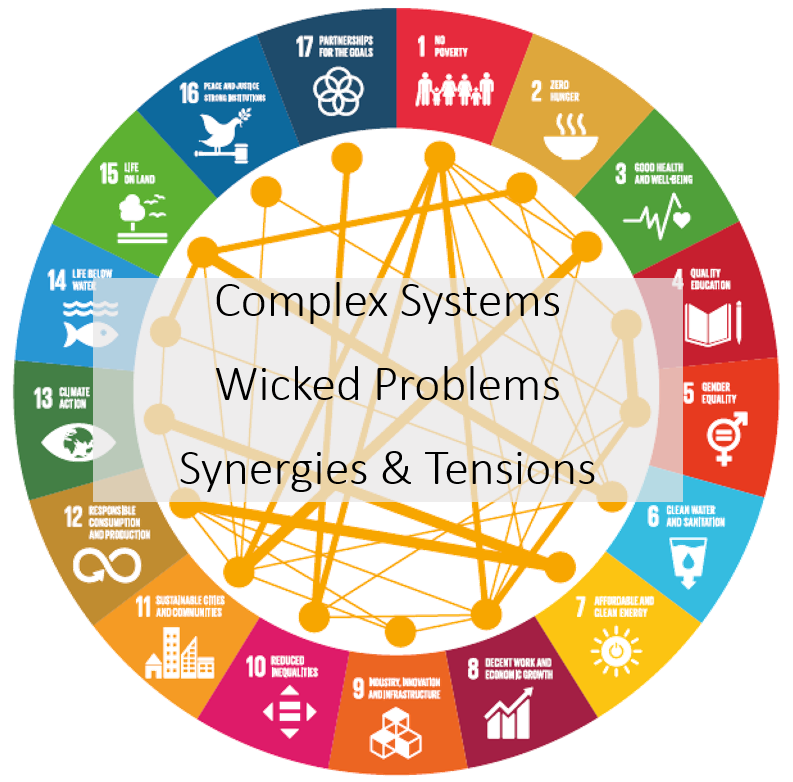
\includegraphics[width=0.45\textwidth]{Imgs/3_complex.PNG}
    \caption{SDGs: Complex and Wicked Planning problems}
    \label{fig:complex_sdg}
\end{figure}
%
Finally, but not least, it is important to recognize that these are not virtual or intangible processes, they occur in specific places in the space. There is reason behind the geographical structure of these events which also deserves to be explored. By introducing the spatial dimension to the analysis, planning for better city-regions, becomes spatial planning. \par

For the purpose of this exposition, the idea that a city is works as a factory will be used to illustrate the general problem being faced here. Now, let's imagine that the owner of a factory wants to increase the amount produced, he would start to ask questions about how much is being currently produced and then start to monitor the amount of inputs requested. By solely looking at these variables, much planning cannot be done. Decisions about the amount and the combination inputs could help to enhance production, but soon more question about the processes behind production will arise. More information about the components of the factory will be requested, number of employees, salaries, energy consumption, machines used, and so forth. As more and more detailed KPIs about the production are being monitored, the processes of production will be revealed. \par

A city is not a a factory. besides many differences, in a factory the processes are linear. Inputs are transformed step by step in a linear process. One step is related to a previous one and so forth. Once a part moves forward in the production line, it never goes back and affects previous process. Social and Economic systems are complex and any performance indicator needs to take into account the complexity of these systems. 

In Rittel and Webber’s \cite{Rittel1973} words 
\begin{quote}
    [large and interconnected network systems] In that structural framework it has become less apparent where problem centers lie, and less apparent where and how we should intervene even if we do happen to know what aims we seek.
\end{quote}\par


Only after unpacking the systems interrelations, it would be possible to meet targets that are sustainable over time and minimize undesirable side effects.\par

Finally, but not least, space must be taken into consideration. Most of these are urban or regional processes occurring in specific locations. Spatial planning, then becomes the tool to help to define the specific set of actions in the space to affect performance.  \par

To sum up, to modify the performance of a complex system it is needed to:


\begin{enumerate}
    \item Understand the processes within the system
    \item Understand how that system interacts with other systems
    \item Understand the spatial-temporal properties 
\end{enumerate}